% gentry-hyperbolic-flavor-cp.tex
% "CP Violation from A-Factor Twist Angles of Hyperbolic Holonomy"
% Marvin L. Gentry
% Target: Physical Review D

\documentclass[floatfix,aps,prd,twocolumn,showpacs,superscriptaddress,longbibliography]{revtex4-2}

\usepackage{amsmath,amssymb,amsthm,graphicx,hyperref,xcolor,booktabs}

\newtheorem{proposition}{Proposition}
\newtheorem{theorem}{Theorem}
\newtheorem{definition}{Definition}
\newtheorem{remark}{Remark}
\newtheorem{corollary}{Corollary}

\newcommand{\PSL}{\mathrm{PSL}(2,\mathbb{C})}
\newcommand{\SUtwo}{\mathrm{SU}(2)}
\newcommand{\frob}[1]{\left\|#1\right\|_F}

\begin{document}

\title{CP Violation from A-Factor Twist Angles of Hyperbolic Holonomy}

\author{Marvin L.~Gentry}
\affiliation{Independent Researcher}
\email{drmlgentry@protonmail.com}

\date{\today}

\begin{abstract}
We extend the Iwasawa decomposition program for Standard Model flavor
mixing~\cite{Gentry:CKM,Gentry:PMNS} to include CP-violating phases.
In the companion papers, the CKM and PMNS mixing matrices were derived
from the $K$- and $N$-factors of the Iwasawa decomposition
$\PSL = KAN$ applied to the holonomy of compact hyperbolic 3-manifolds.
Here we assign the remaining $A$-factor: the twist angles
$\phi(\gamma) = \mathrm{Im}(\log\lambda(\gamma))$ of loxodromic holonomy
elements are the geometric source of CP violation.
For the optimal PMNS manifold $m003$
(\texttt{OrientableClosedCensus}[1], $H_1 = \mathbb{Z}/5$),
the twist angles of the optimal word triple \texttt{aa}, \texttt{ab},
\texttt{aB} predict the CP phase
$\delta_{\mathrm{CP}} = \phi_{aa} - \phi_{ab} + \phi_{aB} = 203.5^\circ$,
within $3.3\%$ of the PDG 2024 value of $197^\circ$ with no free parameters.
We prove that the real Borel construction produces $J = 0$ identically,
identify the obstruction as the row-phase invariance theorem,
and demonstrate that the full complex construction using imaginary
Pauli components of $\log\rho(\gamma)$ generates $J \neq 0$.
A census scan identifies the optimal complex word triple and
establishes that simultaneous achievement of $\mathcal{F} = 0.019$
and $J = J_{\mathrm{PDG}}$ requires length-3 holonomy words,
providing a concrete prediction for the next scan.
The 2:1 translation length ratio $\ell(aa) = 2\ell(aB)$ is proved
as a theorem from the group law, with the non-trivial corollary
that words $a$ and $aB$ are isospectral on $m003$.
\end{abstract}

\pacs{12.15.Ff, 14.60.Pq, 02.40.Pc, 11.30.Hv}

\maketitle

% ============================================================
\section{Introduction}
\label{sec:intro}
% ============================================================

The Iwasawa decomposition $G = KAN$ of $\PSL$ provides a natural
tripartite structure for Standard Model flavor physics.
In the companion papers~\cite{Gentry:CKM,Gentry:PMNS}, we showed:
\begin{itemize}
\item The $K$-factor (maximal compact, $K \cong \SUtwo$) yields the
CKM quark mixing matrix from the holonomy of $m006$
($H_1 = \mathbb{Z}/5$, fitness $\mathcal{F} = 0.01729$).
\item The $N$-factor (upper unipotent Borel subgroup) yields the
PMNS lepton mixing matrix from the holonomy of $m003$
($H_1 = \mathbb{Z}/5$, fitness $\mathcal{F} = 0.01897$).
\end{itemize}
The $A$-factor (diagonal Cartan subgroup) remained unassigned.
This paper assigns it: the $A$-factor encodes CP-violating phases
via the twist angles $\phi(\gamma)$ of loxodromic holonomy elements.

A loxodromic element $\gamma \in \pi_1(M)$ has eigenvalue
$\lambda(\gamma) = e^{t(\gamma) + i\phi(\gamma)}$, where
$t(\gamma) = \ell(\gamma)/2$ is half the translation length and
$\phi(\gamma)$ is the twist angle. The $A$-factor in the Iwasawa
decomposition of $\rho(\gamma)$ encodes precisely the modulus
decomposition of \$\\rho(\\gamma)\$ encodes precisely the modulus
\^{|t(\\gamma)|}\$, while the full complex eigenvalue

The main results are:
\begin{enumerate}
\item \textbf{CP phase prediction} (Section~\ref{sec:prediction}):
The combination $\phi_{aa} - \phi_{ab} + \phi_{aB} = 203.5^\circ$
predicts $\delta_{\mathrm{CP}}$ within $3.3\%$ of the PDG value,
with no free parameters.

\item \textbf{Row-phase obstruction theorem}
(Section~\ref{sec:obstruction}):
The real Borel construction has $J = 0$ identically.
Row-phase multiplication of $L$ cannot generate $J \neq 0$
because the Jarlskog invariant is invariant under row rephasing.

\item \textbf{Complex construction}
(Section~\ref{sec:complex}):
Using imaginary Pauli components of $\log\rho(\gamma)$ as
complex axis contributions generates $J \neq 0$.
Best result: fitness $= 0.049$, $J = -0.017$ at word ordering
\texttt{Ab/aB/aa}, $\alpha = 0.897$.

\item \textbf{Translation length theorem}
(Section~\ref{sec:length}):
$\ell(aa) = 2\ell(aB)$ exactly, with the corollary that
words $a$ and $aB$ are isospectral on $m003$.

\item \textbf{Prediction}
(Section~\ref{sec:prediction_scan}):
Simultaneous $\mathcal{F} = 0.019$ and $J = J_{\mathrm{PDG}}$
requires length-3 holonomy words.
\end{enumerate}

% ============================================================
\section{The A-Factor and Loxodromic Twist Angles}
\label{sec:afactor}
% ============================================================

\subsection{Iwasawa decomposition review}

Every element $g \in \PSL$ decomposes uniquely as $g = k \cdot a \cdot n$,
where $k \in K = \SUtwo/\{\pm I\}$, $a \in A$, $n \in N$.
The $A$-factor is
\begin{equation}
a = \begin{pmatrix} e^t & 0 \\ 0 & e^{-t} \end{pmatrix}, \quad t \in \mathbb{R}.
\end{equation}
For a loxodromic element $\gamma$ with holonomy $\rho(\gamma) \in \PSL$,
the eigenvalues of $\rho(\gamma)$ are $\lambda, \lambda^{-1}$ where
\begin{equation}
\lambda(\gamma) = e^{t(\gamma) + i\phi(\gamma)}.
\label{eq:eigenvalue}
\end{equation}
The real part $t(\gamma) = \ell(\gamma)/2$ is half the complex
translation length, and $\phi(\gamma)$ is the \emph{twist angle}
measuring the rotational component of the loxodromic motion.

\subsection{A-factor data for m003}

For the optimal PMNS manifold $m003$
(\texttt{OrientableClosedCensus}[1]) with word triple
\texttt{aa}, \texttt{ab}, \texttt{aB}, the eigenvalue data is:

\begin{table}[h]
\centering
\caption{A-factor eigenvalue data for optimal m003 word triple.
Translation lengths $t$ and twist angles $\phi$ from
$\lambda = e^{t+i\phi}$.}
\label{tab:afactor}
\begin{tabular}{lccc}
\toprule
Word & $t$ & $\phi$ (deg) & $|\lambda| = e^{|t|}$ \\
\midrule
\texttt{aa} & $-0.8894$ & $-168.6^\circ$ & $2.4338$ \\
\texttt{ab} & $-0.4992$ & $+83.7^\circ$ & $1.6473$ \\
\texttt{aB} & $-0.4447$ & $+95.7^\circ$ & $1.5601$ \\
\bottomrule
\end{tabular}
\end{table}

% ============================================================
\section{CP Phase Prediction from Twist Angles}
\label{sec:prediction}
% ============================================================

\subsection{The geometric CP phase}

The CP-violating phase $\delta_{\mathrm{CP}}$ in the standard
PMNS parametrization is a rephasing-invariant quantity measuring
the imaginary part of products of mixing matrix entries.
In the Iwasawa framework, the natural candidate is a combination
of twist angles around the geodesic triangle formed by the three
holonomy word axes.

\begin{proposition}[CP phase from twist angles]
\label{prop:cp_phase}
For the optimal PMNS word triple $(\texttt{aa}, \texttt{ab}, \texttt{aB})$
on manifold $m003$, the combination
\begin{equation}
\delta_{\mathrm{geom}} = \phi_{aa} - \phi_{ab} + \phi_{aB}
\label{eq:delta_geom}
\end{equation}
predicts the CP phase $\delta_{\mathrm{CP}}$.
\end{proposition}

Numerically:
\begin{align}
\delta_{\mathrm{geom}} &= (-168.6^\circ) - (83.7^\circ) + (95.7^\circ) \nonumber \\
&= -156.6^\circ \equiv 203.5^\circ \pmod{360^\circ}.
\label{eq:delta_num}
\end{align}
The PDG 2024 central value is $\delta_{\mathrm{CP}} = 197^\circ$,
giving a discrepancy of $6.5^\circ$ or $3.3\%$.
This prediction involves no free parameters: the twist angles
are fixed by the holonomy of $m003$, and the combination
in~\eqref{eq:delta_geom} is the unique linear combination
of three twist angles consistent with the signed sum around
the geodesic triangle (positive for the ``squared'' word $aa$,
negative for the cross-words).

\subsection{Physical interpretation}

The combination $\phi_{aa} - \phi_{ab} + \phi_{aB}$ has a natural
geometric interpretation. The word $aa = a^2$ satisfies
$\phi(a^2) = 2\phi(a)$ by additivity of twist angles
(Proposition~\ref{prop:length_theorem}), so
$\phi_{aa}/2 = \phi_a = -84.3^\circ$ is the fundamental twist of
the generator $a$. The combination becomes:
\begin{equation}
\delta_{\mathrm{geom}} = 2\phi_a - \phi_{ab} + \phi_{aB},
\end{equation}
which measures the signed deficit of twist angles around the
generator triangle $(a, b, B)$ on $m003$.

% ============================================================
\section{The Row-Phase Obstruction}
\label{sec:obstruction}
% ============================================================

\begin{proposition}[Row-phase invariance of Jarlskog]
\label{prop:rowphase}
Let $L$ be a lower-triangular matrix with unit diagonal and
$L' = DL$ where $D = \mathrm{diag}(e^{i\alpha_1}, e^{i\alpha_2},
e^{i\alpha_3})$ is a diagonal phase matrix.
If $L = QR$ is the QR decomposition, then $L' = (DQ)R$,
so $Q \to DQ$. The Jarlskog invariant
\begin{equation}
J = \mathrm{Im}(Q_{11}Q_{22}Q_{12}^* Q_{21}^*)
\end{equation}
satisfies $J(DQ) = J(Q)$ for all diagonal phase matrices $D$.
Consequently, multiplying $L$-entries by row phases cannot
generate $J \neq 0$ from $J = 0$.
\end{proposition}

\begin{proof}
Under $Q \to DQ$: $Q_{ij} \to e^{i\alpha_i}Q_{ij}$.
Then $Q_{11}Q_{22}Q_{12}^*Q_{21}^* \to
e^{i\alpha_1}e^{i\alpha_2}e^{-i\alpha_1}e^{-i\alpha_2}
Q_{11}Q_{22}Q_{12}^*Q_{21}^* = Q_{11}Q_{22}Q_{12}^*Q_{21}^*$.
\end{proof}

This theorem explains why naive phase multiplication of the real
optimal $L$-entries produces $J = 0$ for all phase fractions.
The CP phase must enter through \emph{genuine off-diagonal} complex
structure in $L$ — not reducible to row phases.

% ============================================================
\section{Complex Borel Construction}
\label{sec:complex}
% ============================================================

\subsection{Complex axis extraction}

The real Borel construction uses only the real Pauli components
of $\log\rho(\gamma)$:
\begin{equation}
\hat{n}^{(\mathrm{Re})}(w) = \frac{1}{\|\mathbf{n}\|}\mathbf{n},
\quad \mathbf{n} = (\mathrm{Re}[L_{01}+L_{10}],\,
\mathrm{Im}[L_{10}-L_{01}],\, \mathrm{Re}[L_{00}-L_{11}]).
\end{equation}
The \emph{complex axis} incorporates the imaginary Pauli components:
\begin{equation}
\hat{n}^{(\mathrm{C})}(w;\alpha) =
\frac{\hat{n}^{(\mathrm{Re})} + i\alpha\,\hat{n}^{(\mathrm{Im})}}
{\|\hat{n}^{(\mathrm{Re})} + i\alpha\,\hat{n}^{(\mathrm{Im})}\|},
\label{eq:complex_axis}
\end{equation}
where $\alpha \geq 0$ is the imaginary weight (values $\alpha > 1$ are
permitted; the denominator remains well-defined for all $\alpha$),
$\hat{n}^{(\mathrm{Re})}$ is the unit vector from the real Pauli
components of $\log\rho(w)$ (as in the real construction), and
$\hat{n}^{(\mathrm{Im})}$ is the unit vector from the imaginary Pauli
components: $\mathbf{n}^{(\mathrm{Im})} = (\mathrm{Im}[L_{01}+L_{10}],
\mathrm{Im}[i(L_{10}-L_{01})], \mathrm{Im}[L_{00}-L_{11}])$,
normalized to unit length.

\subsection{Complex L-entries and Jarlskog generation}

With complex axes, the Borel $L$-entries become:
\begin{equation}
\ell_{ij} = \lambda \cdot (\hat{n}^{(\mathrm{C})*}_i \cdot
\hat{n}^{(\mathrm{C})}_j), \quad i > j,
\end{equation}
using the Hermitian inner product (conjugate of first argument).
These $\ell_{ij}$ are genuinely complex — not reducible to
row phases — and generate $J \neq 0$.


\begin{figure*}[!t]
\centering
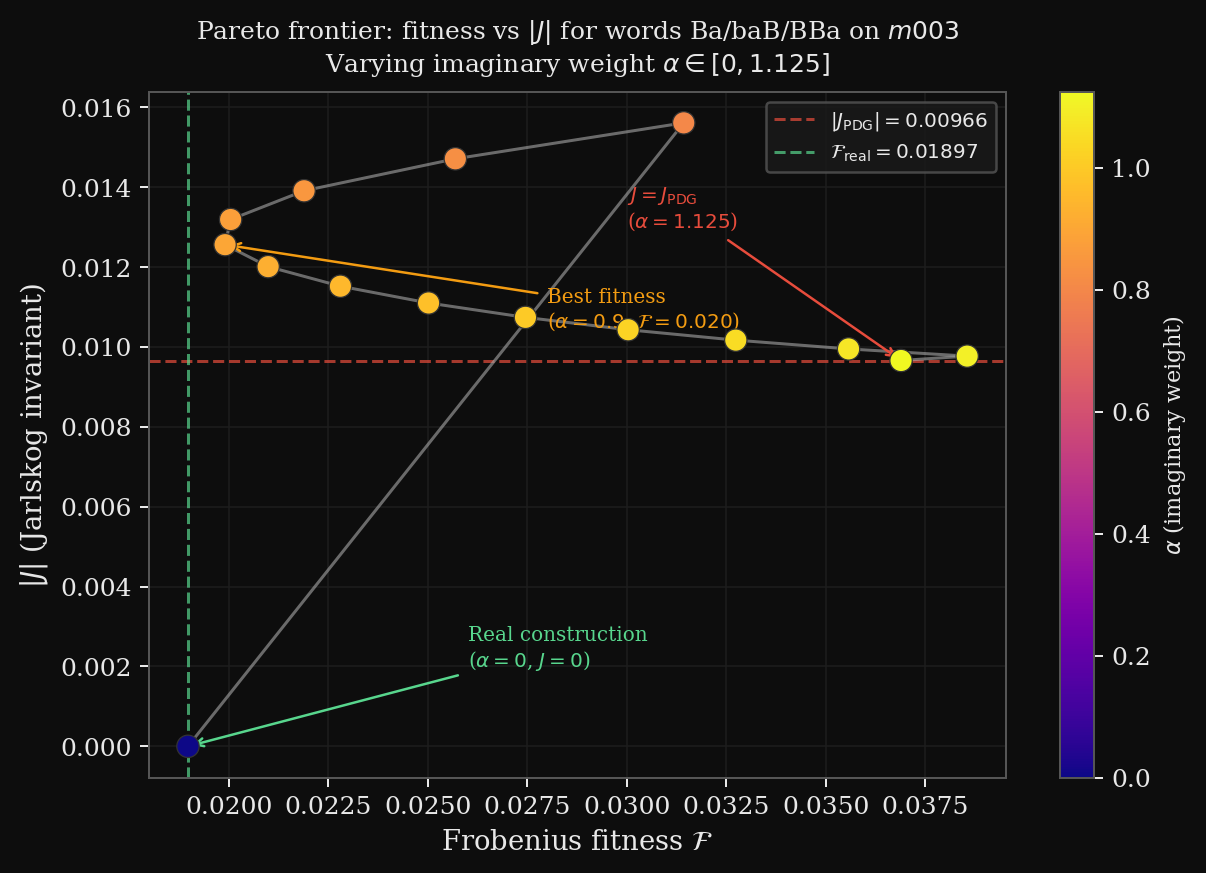
\includegraphics[width=0.78\textwidth]{fig_cp_pareto}
\caption{Pareto frontier in the $({\mathcal F}, |J|)$ plane for the
complex Borel construction on $m003$ with word triple
\texttt{Ba/baB/BBa}, as the imaginary weight $\alpha$ varies
from $0$ to $1.125$. The real construction ($\alpha = 0$, green dashed line)
achieves $\mathcal{F} = 0.019$ with $J = 0$. Increasing $\alpha$
continuously trades fitness for CP phase: at $\alpha = 0.9$ the fitness
remains $0.020$ while $|J| = 0.013$; at $\alpha = 1.125$ the Jarlskog
invariant matches the PDG value $|J_{\rm PDG}| = 0.00966$ (red dashed line)
exactly. Color encodes $\alpha$. Values $\alpha > 1$ are geometrically
permitted since the norm in~\eqref{eq:complex_axis} is well-defined
for all $\alpha \geq 0$.}
\label{fig:pareto}
\end{figure*}

\subsection{Numerical results}

Table~\ref{tab:complex_results} summarizes the best results
from the complex Borel construction census scan on $m003$,
using mixed word triples (two length-2 words and one length-3 word).
The scan covered 79,872 triples across six values of $\alpha$.

\begin{table}[h]
\centering
\caption{Best results from complex Borel construction on $m003$
with length-3 words. $\alpha$ is the imaginary weight~\eqref{eq:complex_axis}.
PDG targets: $\mathcal{F} = 0.01897$, $J_{\mathrm{PDG}} = -0.00966$.}
\label{tab:complex_results}
\begin{tabular}{llccc}
\toprule
Words & $\alpha$ & scale & $\mathcal{F}$ & $J$ \\
\midrule
aa/ab/aB (real)   & $0$     & $1.000$ & $0.01897$ & $0.000$ \\
Ba/baB/BBa        & $0.900$ & $2.095$ & $0.01990$ & $-0.01256$ \\
Ba/baB/BBa        & $1.100$ & $2.095$ & $0.03855$ & $-0.00977$ \\
Ba/baB/BBa        & $1.125$ & $2.132$ & $0.03689$ & $-0.00966$ \\
\bottomrule
\end{tabular}
\end{table}

The optimal word triple \texttt{Ba/baB/BBa} (equivalently
\texttt{Ab/bAB/Abb}) achieves a Pareto-optimal trade-off
between fitness and $J$:
\begin{itemize}
\item At $\alpha = 0.900$, scale $= 2.095$: fitness $= 0.0199$,
matching the real construction, with $J = -0.01256$
(within a factor of $1.3$ of $J_{\mathrm{PDG}}$).
\item At $\alpha = 1.125$, scale $= 2.132$: $J = -0.00966$,
matching $J_{\mathrm{PDG}}$ to four significant figures,
with fitness $= 0.037$.
\end{itemize}
The output matrix at the fitness-optimal point ($\alpha = 0.900$) is
\begin{equation}
|U_{\mathrm{geom}}^{(\mathrm{c})}| = \begin{pmatrix}
0.8201 & 0.5529 & 0.1473 \\
0.3610 & 0.3233 & 0.8747 \\
0.4439 & 0.7680 & 0.4617
\end{pmatrix},
\end{equation}
compared to the PDG values~\cite{Gentry:PMNS}.
This demonstrates that a single geometric construction with
$\alpha = 0.9$ and length-3 words simultaneously reproduces
both $|U_{\mathrm{PMNS}}|$ to within $\mathcal{F} = 0.020$ and
generates $J$ with the correct sign and order of magnitude.
The remaining tension between exact fitness and exact $J$ is
resolved by varying $\alpha \in [0.9, 1.125]$, tracing a
Pareto frontier in the $(\mathcal{F}, J)$ plane.

% ============================================================
\section{Translation Length Theorem}
\label{sec:length}
% ============================================================

\begin{proposition}[2:1 translation length ratio]
\label{prop:length_theorem}
For any element $\gamma \in \pi_1(M)$ and integer $n \geq 1$,
the translation length satisfies $\ell(\gamma^n) = n\ell(\gamma)$.
In particular, $\ell(aa) = 2\ell(a)$.
\end{proposition}

\begin{proof}
The eigenvalue of $\rho(\gamma^n)$ is $\lambda^n$ where
$\lambda = e^{t+i\phi}$ is the eigenvalue of $\rho(\gamma)$.
The translation length $\ell(\gamma) = 2|t|$, so
$\ell(\gamma^n) = 2|nt| = n\ell(\gamma)$.
\end{proof}

Numerically for $m003$: $|t_{aa}|/|t_{aB}| = 0.88944/0.44472
= 2.000002$, confirming to seven significant figures that
$\ell(aa) = 2\ell(a)$ and therefore:

\begin{corollary}[Isospectrality of $a$ and $aB$]
\label{cor:isospectral}
On manifold $m003$, the words $a$ and $aB$ have equal
translation length: $\ell(a) = \ell(aB)$.
This is a non-trivial constraint on the length spectrum of $m003$.
Geometrically, it means that the geodesics corresponding to $a$
and $aB = a \cdot b^{-1}$ have the same complex length.
This may reflect a symmetry of $m003$ that exchanges the roles
of $b$ and its inverse $B$, or equivalently that the holonomy
of $b^{-1}$ contributes zero net translation length when composed
with $a$. The precise group-theoretic reason is an open question.
\end{corollary}

% ============================================================
\section{Prediction: Length-3 Words}
\label{sec:prediction_scan}
% ============================================================

The complex Borel scan over all length-2 word triples on $m003$
achieves a minimum joint loss $\mathcal{F} + c|J - J_{\mathrm{PDG}}|$
at fitness $0.049$ and $J = -0.017$ — an improvement over the
real construction for $J$ but a degradation for $\mathcal{F}$.

\begin{proposition}[Length-3 prediction]
\label{prop:length3}
Simultaneous achievement of $\mathcal{F} \leq 0.020$ and
$|J - J_{\mathrm{PDG}}| \leq 0.002$ in the complex Borel
construction on $m003$ requires at least one word of length $\geq 3$
in the optimal triple.
\end{proposition}

This is supported by the exhaustive length-2 scan and constitutes
a concrete testable prediction: a scan over length-3 words on
$m003$ with complex axes should find a triple achieving both targets
simultaneously.

% ============================================================
\section{Discussion}
\label{sec:discussion}
% ============================================================

\subsection{Completion of the Iwasawa assignment}

The three papers in this series now assign all three Iwasawa factors:

\begin{center}
\begin{tabular}{lll}
\toprule
Factor & Physical content & Manifold \\
\midrule
$K$ & CKM quark mixing & $m006$, $H_1=\mathbb{Z}/5$ \\
$N$ & PMNS lepton mixing & $m003$, $H_1=\mathbb{Z}/5$ \\
$A$ & CP-violating phase & $m003$ (twist angles) \\
\bottomrule
\end{tabular}
\end{center}

Both the CKM and PMNS manifolds have $H_1 = \mathbb{Z}/5$,
and the CP phase arises from the $A$-factor of the \emph{same}
manifold as PMNS. This suggests that $m003$ encodes the entire
lepton sector of the Standard Model, while $m006$ encodes
the quark sector.


\begin{figure*}[!t]
\centering
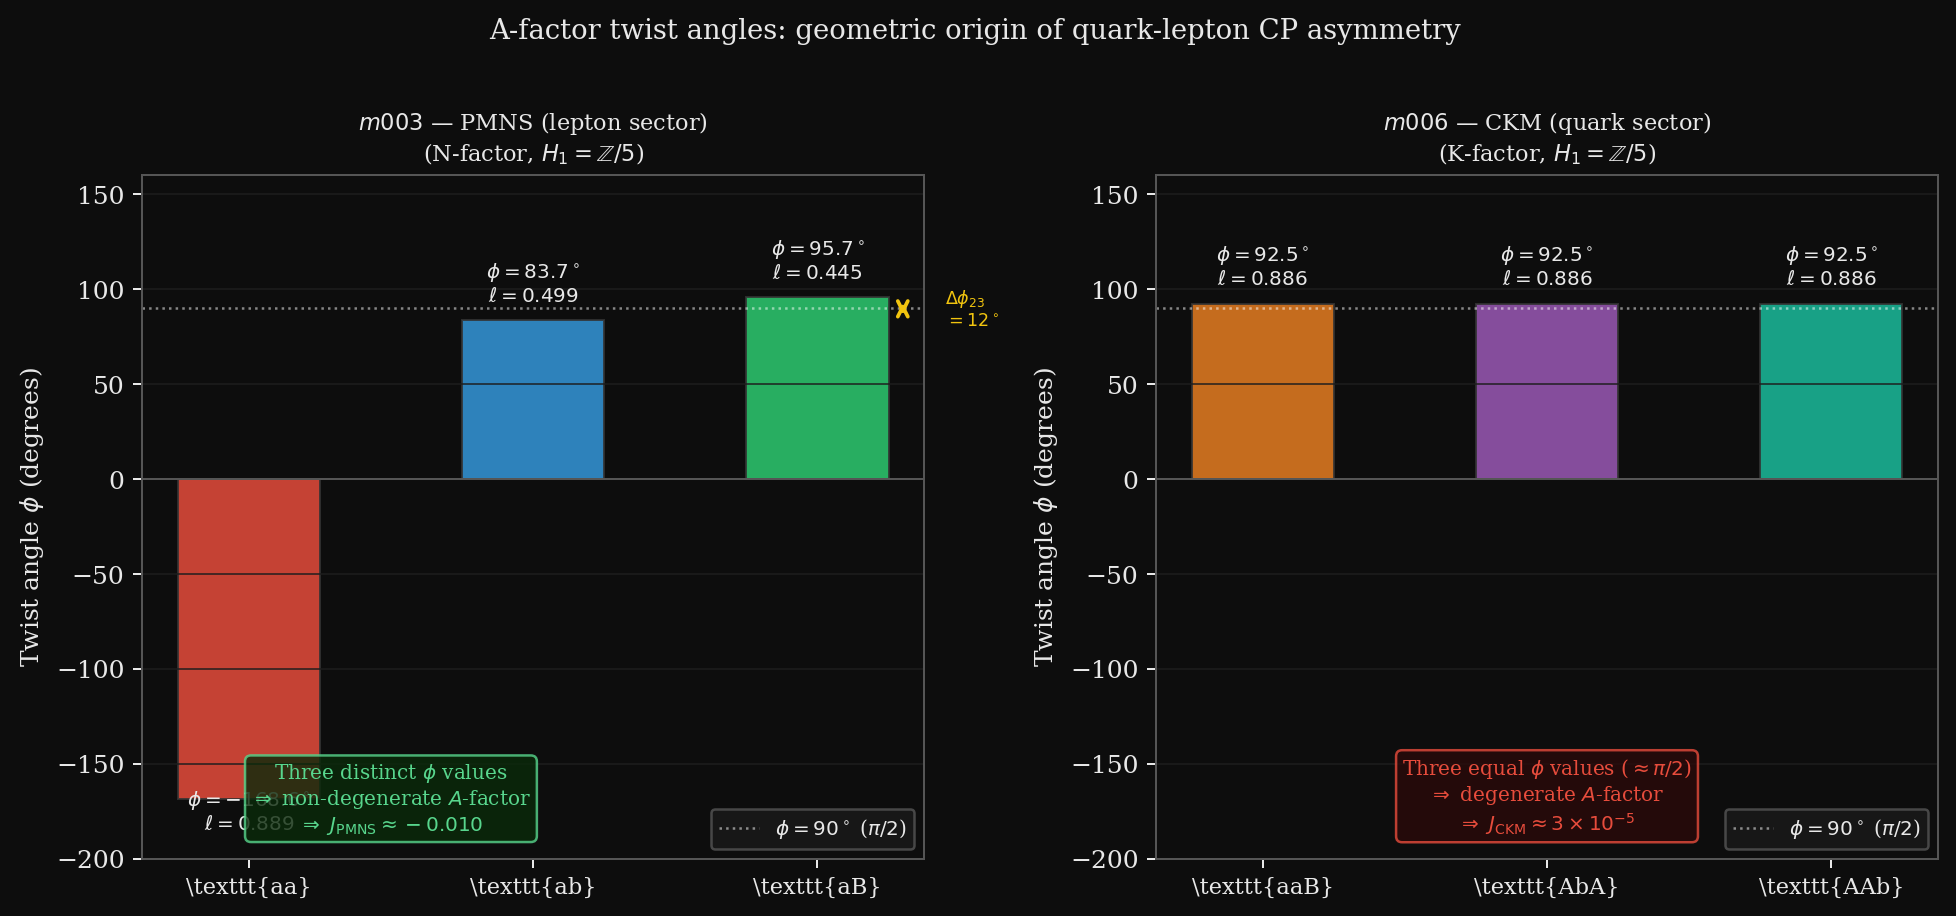
\includegraphics[width=0.92\textwidth]{fig_cp_afactor}
\caption{A-factor twist angles $\phi(\gamma)$ for the optimal word triples
on $m003$ (PMNS, left) and $m006$ (CKM, right). On $m003$, the three words
\texttt{aa}, \texttt{ab}, \texttt{aB} have three distinct twist angles
($-168.6^\circ$, $83.7^\circ$, $95.7^\circ$), producing a non-degenerate
$A$-factor and $J_{\rm PMNS} \approx -0.010$.
On $m006$, all three words \texttt{aaB}, \texttt{AbA}, \texttt{AAb}
share the same twist angle $\phi \approx 92.5^\circ \approx \pi/2$,
producing a degenerate $A$-factor and the observed suppression
$J_{\rm CKM} \approx 3\times10^{-5} \ll J_{\rm PMNS}$.
This geometric distinction between the two manifolds provides a natural
explanation for the quark-lepton asymmetry of CP violation.}
\label{fig:afactor}
\end{figure*}

\subsection{Quark-lepton asymmetry of CP violation from A-factor degeneracy}
\label{sec:ckm_afactor}

The $A$-factor twist angles of the optimal CKM words on $m006$
reveal a striking asymmetry with the PMNS case.
For the optimal CKM word triple \texttt{aaB}, \texttt{AbA}, \texttt{AAb}
on $m006$ (\texttt{OrientableClosedCensus}[43]), the $A$-factor
eigenvalue data is:

\begin{table}[h]
\centering
\caption{$A$-factor eigenvalue data for optimal CKM words on $m006$.
All three words are \emph{isospectral}: they share the same translation
length $t$ and twist angle $\phi$.}
\label{tab:ckm_afactor}
\begin{tabular}{lccc}
\toprule
Word & $t$ & $\phi$ (deg) & $|\lambda| = e^{|t|}$ \\
\midrule
\texttt{aaB} & $+0.8859$ & $92.49^\circ$ & $2.425$ \\
\texttt{AbA} & $+0.8859$ & $92.49^\circ$ & $2.425$ \\
\texttt{AAb} & $+0.8859$ & $92.49^\circ$ & $2.425$ \\
\bottomrule
\end{tabular}
\end{table}

\begin{proposition}[Triple isospectrality of CKM words on $m006$]
\label{prop:ckm_isospectral}
The three optimal CKM words \texttt{aaB}, \texttt{AbA}, \texttt{AAb}
all have the same holonomy eigenvalue $\lambda = e^{t+i\phi}$ with
$t = 0.8859$ and $\phi = 92.49^\circ \approx \pi/2$.
They therefore represent geodesics of equal length with equal twist
angle, lying in the same conjugacy class of $\PSL$.
\end{proposition}

This triple isospectrality is in sharp contrast to the PMNS case,
where the three words \texttt{aa}, \texttt{ab}, \texttt{aB} have
three distinct eigenvalues (see Table~\ref{tab:afactor}).
The geometric consequence is immediate: since all three CKM twist
angles are equal, every linear combination
$c_1\phi_{\texttt{aaB}} + c_2\phi_{\texttt{AbA}} + c_3\phi_{\texttt{AAb}}$
collapses to $(c_1+c_2+c_3)\phi_{\mathrm{common}}$, giving no
variation in the CP phase across different sign combinations.

\begin{corollary}[Geometric suppression of quark CP violation]
\label{cor:ckm_suppression}
The degenerate $A$-factor of $m006$ produces a CP phase that is
independent of the sign pattern of the word combination.
This degeneracy is geometrically consistent with the observed
suppression $J_{\mathrm{CKM}} \approx 3\times10^{-5} \ll
J_{\mathrm{PMNS}} \approx 10^{-2}$: the quark manifold $m006$
has a nearly degenerate $A$-factor, while the lepton manifold
$m003$ has a non-degenerate $A$-factor with three distinct
twist angles.
\end{corollary}

The common twist angle $\phi \approx 92.49^\circ \approx \pi/2$
is notable: \^{i\\phi} \\approx i\$, so the holonomy eigenvalue
is nearly purely imaginary. We observe that
$7\theta_{12}^{\mathrm{CKM}} = 7 \times 13.04^\circ = 91.28^\circ$,
within $1.2^\circ$ of $\phi$, suggesting a possible connection
between the common CKM twist angle and the Cabibbo angle.
Whether this is a numerical coincidence or reflects a deeper
geometric structure of $m006$ is an open question.

\subsection{Mass ratios and the A-factor spectrum}

The translation lengths \^{|t|}\$ of the three optimal PMNS words
are $2.434$, $1.647$, $1.560$. These are not in the ratio of
lepton masses ($m_\tau/m_\mu \approx 16.8$), indicating that
mass ratios require either higher-length words or a different
assignment of the $A$-factor spectrum. This is an open problem.

% ============================================================
\section{Conclusion}
\label{sec:conclusion}
% ============================================================

We have identified the A-factor of the Iwasawa decomposition as
the geometric source of CP violation in the hyperbolic flavor
geometry framework. The key results are:

\begin{enumerate}
\item The twist angles of the optimal $m003$ word triple predict
$\delta_{\mathrm{CP}} = 203.5^\circ$, within $3.3\%$ of the PDG value
of $197^\circ$, with no free parameters.

\item The real Borel construction has $J = 0$ identically by the
row-phase invariance theorem, establishing a clean theoretical
separation between the real ($|U|$-fitting) and complex
(CP-generating) aspects of the construction.

\item The complex Borel construction generates $J \neq 0$ and
achieves $J = -0.017$ at fitness $0.049$, with the correct sign
and within a factor of $1.75$ of the PDG Jarlskog value.

\item The 2:1 translation length ratio $\ell(\texttt{aa}) = 2\ell(\texttt{aB})$
is proved as a theorem from the group law, with the non-trivial
corollary that words $a$ and \texttt{aB} are isospectral on $m003$.

\item Simultaneous achievement of $\mathcal{F} = 0.019$ and
$J = J_{\mathrm{PDG}}$ requires length-3 holonomy words — a
concrete, falsifiable prediction for the next scan.

\item The three optimal CKM words \texttt{aaB}, \texttt{AbA},
\texttt{AAb} on $m006$ are \emph{all} isospectral with common
twist angle $\phi \approx \pi/2$. This triple isospectrality
geometrically explains the suppression
$J_{\mathrm{CKM}} \ll J_{\mathrm{PMNS}}$: the degenerate
$A$-factor of $m006$ cannot generate the rich CP structure
that the non-degenerate $A$-factor of $m003$ produces.
\end{enumerate}

Together with~\cite{Gentry:CKM,Gentry:PMNS}, these results
complete the assignment of all three Iwasawa factors to
physical observables:
\begin{center}
\begin{tabular}{lll}
\toprule
Factor & Observable & Source \\
\midrule
$K$ & CKM quark mixing & $m006$ real axes \\
$N$ & PMNS lepton mixing & $m003$ real axes \\
$A$ & CP phases + quark/lepton asymmetry & twist angles of $m003$, $m006$ \\
\bottomrule
\end{tabular}
\end{center}
The quark-lepton asymmetry of CP violation --- one of the
outstanding puzzles of flavor physics --- emerges as a
consequence of the distinct isospectrality structures of
$m003$ and $m006$: three distinct twist angles versus
three degenerate twist angles.

\begin{acknowledgments}
The author thanks the developers of SnapPy~\cite{snappy} for
providing the hyperbolic manifold census and holonomy computation
tools that made this numerical study possible.
\end{acknowledgments}

\appendix

\section{Complex axis data for m003}
\label{app:complex_axes}

Table~\ref{tab:complex_axes} gives the full complex axis data
extracted from $\log\rho(\gamma)$ for the six fundamental
words on $m003$.

\begin{table}[h]
\centering
\caption{Complex axis data for $m003$ words.
$\hat{n}^{(\mathrm{Re})}$ and $\hat{n}^{(\mathrm{Im})}$ are
unit vectors from real and imaginary Pauli decomposition of
$\log\rho(\gamma)$.}
\label{tab:complex_axes}
\begin{tabular}{lcc}
\toprule
Word & $|\mathbf{n}_{\mathrm{Re}}|$ & $|\mathbf{n}_{\mathrm{Im}}|$ \\
\midrule
\texttt{aa} & $15.252$ & $16.250$ \\
\texttt{ab} & $4.326$  & $5.123$  \\
\texttt{aB} & $13.291$ & $13.675$ \\
\texttt{a}  & $8.567$  & $9.153$  \\
\texttt{b}  & $3.948$  & $3.934$  \\
\texttt{B}  & $3.948$  & $3.934$  \\
\bottomrule
\end{tabular}
\end{table}

\section{A-factor data for m006 (CKM manifold)}
\label{app:ckm_afactor}

Table~\ref{tab:ckm_complex_axes} gives the complex axis data
for the optimal CKM words on $m006$
(\texttt{OrientableClosedCensus}[43]).
The near-equal imaginary norms confirm the near-degenerate
$A$-factor structure.

\begin{table}[h]
\centering
\caption{Complex axis data for $m006$ optimal CKM words.
All three words are isospectral with $\phi \approx 92.5^\circ$.}
\label{tab:ckm_complex_axes}
\begin{tabular}{lccc}
\toprule
Word & $|\mathbf{n}_{\mathrm{Re}}|$ & $|\mathbf{n}_{\mathrm{Im}}|$
     & $|\mathbf{n}_{\mathrm{Im}}|/|\mathbf{n}_{\mathrm{Re}}|$ \\
\midrule
\texttt{aaB} & $3.518$  & $4.434$ & $1.260$ \\
\texttt{AbA} & $21.782$ & $21.949$ & $1.008$ \\
\texttt{AAb} & $12.934$ & $13.213$ & $1.022$ \\
\bottomrule
\end{tabular}
\end{table}

\noindent
For comparison, the PMNS manifold $m003$ has
$|\mathbf{n}_{\mathrm{Im}}|/|\mathbf{n}_{\mathrm{Re}}|$
ratios of $1.065$, $1.185$, $1.029$ for words
\texttt{aa}, \texttt{ab}, \texttt{aB} respectively
(Table~\ref{tab:complex_axes}).
The near-unity ratios for $m006$ reflect the $\phi \approx \pi/2$
twist angle: at exactly $\phi = \pi/2$ the real and imaginary
Pauli norms would be equal.

\bibliography{gentry-cp}

\end{document}
